\chapter{Stratégie de synthèse et chimie verte}\label{ch:g12:synthesis-strategy}

Un même antidouleur, l'ibuprofène, a été fabriqué de deux façons.
L'ancienne voie compte six étapes, et sur cent kilogrammes de \omterm{def:g7:chemical-reactions:reactant}{réactifs}
achetés, soixante finissent en déchets. La nouvelle compte trois étapes,
et conserve presque chaque \omterm{def:g7:atoms-and-molecules:atom}{atome} acheté. Les deux donnent la même poudre
blanche dans le comprimé~; elles diffèrent par leur conception. Un
chimiste qui planifie une \omterm{def:g10:synthesis-yield:synthesis}{synthèse} se pose quatre questions~: comment
aller vite, comment obtenir beaucoup, comment ne toucher que la bonne
partie d'une \omterm{def:g7:atoms-and-molecules:molecule}{molécule}, et comment gaspiller peu.

\begin{recall}
Une \omterm{def:g10:synthesis-yield:synthesis}{synthèse}~: réaction, séparation, purification, identification~; son
\omterm{def:g10:synthesis-yield:yield}{rendement} (\cref{ch:g10:synthesis-yield}). Les \omterm{def:g12:curly-arrows:curly-arrow}{flèches courbes}, la
\omterm{def:g12:curly-arrows:categories}{substitution}, l'\omterm{def:g12:curly-arrows:categories}{addition}, l'\omterm{def:g12:curly-arrows:categories}{élimination} (\cref{ch:g12:curly-arrows}).
Un \omterm{def:g12:catalysis:catalyst}{catalyseur} accélère une réaction sans être consommé
(\cref{ch:g12:catalysis}). Une \omterm{def:g12:equilibrium:non-total}{réaction non totale} s'arrête quand
$Q = K$~; un excès d'un \omterm{def:g7:chemical-reactions:reactant}{réactif}, ou l'élimination d'un produit, la fait
progresser davantage (\cref{ch:g12:equilibrium}).
\end{recall}

\begin{omfigure}
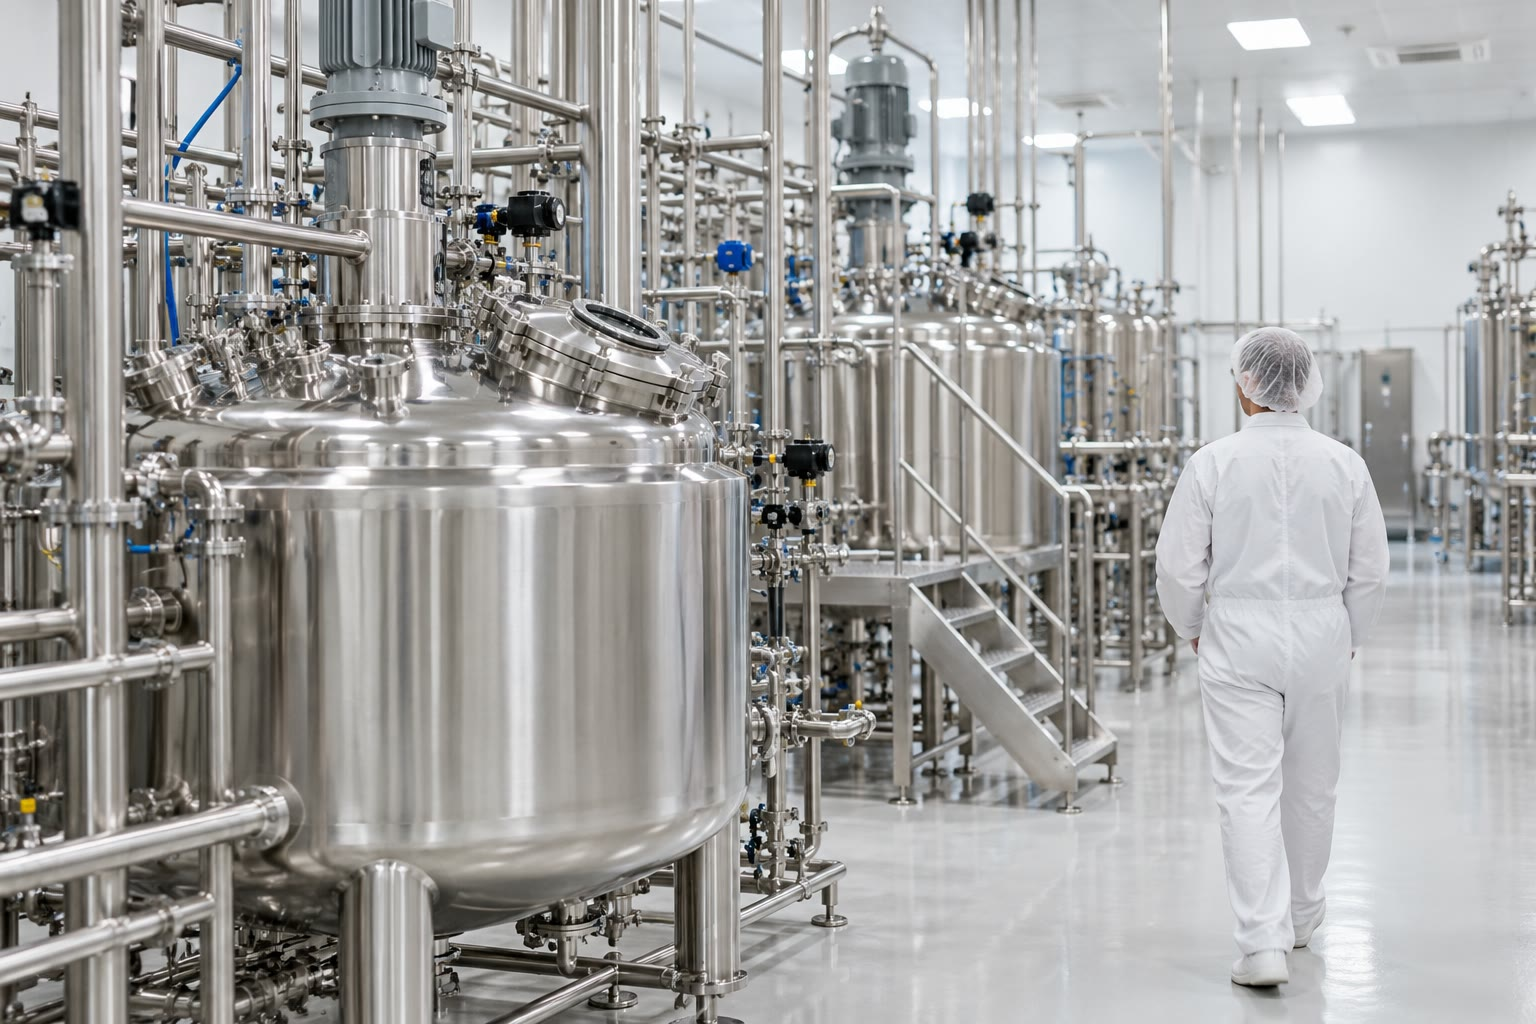
\includegraphics[width=0.48\linewidth]{images/book1/ai/g12-pharma-plant.jpg}

{\small Une usine pharmaceutique~: les réacteurs d'une \omterm{def:g10:synthesis-yield:synthesis}{synthèse}, à
l'échelle de la tonne.}
\end{omfigure}

\section{Optimiser une synthèse}

On peut améliorer deux choses différentes~: la \emph{vitesse}, qui
décide de la durée de la \omterm{def:g10:synthesis-yield:synthesis}{synthèse}, et le \emph{\omterm{def:g10:synthesis-yield:yield}{rendement}}, qui décide de
la quantité de produit obtenue.

\begin{proposition}[Les leviers sur la vitesse et le rendement]\label{prop:g12:synthesis-strategy:levers}
\begin{itemize}
  \item La vitesse augmente avec la température, avec les concentrations
        des \omterm{def:g7:chemical-reactions:reactant}{réactifs}, et avec un \omterm{def:g12:catalysis:catalyst}{catalyseur}.
  \item Le \omterm{def:g10:synthesis-yield:yield}{rendement} final d'une \omterm{def:g10:reaction-progress-table:limiting}{réaction totale} est fixé par le \omterm{def:g10:reaction-progress-table:limiting}{réactif
        limitant}~; celui d'une \omterm{def:g12:equilibrium:non-total}{réaction non totale} augmente avec un excès
        de l'un des \omterm{def:g7:chemical-reactions:reactant}{réactifs}, ou avec l'élimination d'un produit au fur et
        à mesure de sa formation. Un \omterm{def:g12:catalysis:catalyst}{catalyseur} ne le modifie pas~: il ne
        fait qu'amener plus vite le système au même \omterm{def:g10:reaction-progress-table:system}{état final}.
\end{itemize}
\end{proposition}

\begin{proof}
Le premier point rassemble les \omterm{def:g12:reaction-rates:kinetic-factor}{facteurs cinétiques} des
\cref{ch:g12:reaction-rates,ch:g12:catalysis}. Le second découle de
$Q = K$ à la fin d'une \omterm{def:g12:equilibrium:non-total}{réaction non totale}~: ajouter un \omterm{def:g7:chemical-reactions:reactant}{réactif} ou
retirer un produit rend $Q < K$, et la réaction se poursuit dans le sens
direct.
\end{proof}

\begin{example}[L'estérification avec un piège à eau]\label{ex:g12:synthesis-strategy:trap}
L'acide éthanoïque et l'éthanol, une \omterm{def:g10:the-mole:amount}{mole} de chaque, ne donnent que
\qty{67}{\percent} d'\omterm{def:g11:functional-groups:carboxylic-acid}{ester} à l'équilibre. Si l'on chauffe le \omterm{def:g6:pure-substances-and-mixtures:mixture}{mélange} à
reflux dans un \omterm{def:g6:solutions-and-solubility:solute}{solvant} \omterm{def:g6:solutions-and-solubility:miscible}{non miscible} à l'eau, avec un peu d'acide comme
\omterm{def:g12:catalysis:catalyst}{catalyseur}, la vapeur se condense dans un tube latéral, un \emph{piège à
eau} (appareil de Dean-Stark)~: l'eau, plus dense, se rassemble au fond
et y reste, tandis que le \omterm{def:g6:solutions-and-solubility:solute}{solvant} retourne dans le ballon. L'eau quitte
la réaction au fur et à mesure qu'elle se forme, $Q$ reste inférieur à
$K$, et l'estérification devient presque totale. Le chauffage apporte la
vitesse, le \omterm{def:g12:catalysis:catalyst}{catalyseur} davantage de vitesse, le piège le \omterm{def:g10:synthesis-yield:yield}{rendement}.
\end{example}

\begin{omfigure}
\begin{tikzpicture}[font=\small, scale=0.8]
  \pic[transform shape] at (0,0) {hotplate};
  \pic[transform shape] at (0,0) {rbflask={0.55}{orange!20}};
  % the trap: water at the bottom, solvent above, up to the arm
  \fill[cyan!60!blue!40] (1.0,1.75) arc[start angle=180, end angle=360, radius=0.15] -- (1.3,2.3) -- (1.0,2.3) -- cycle;
  \fill[yellow!35] (1.0,2.3) rectangle (1.3,3.25);
  \draw[om glass] (-0.2,3.0) -- (-0.2,3.75) -- (0.2,3.75) -- (0.2,3.55) -- (1.0,3.55) -- (1.0,4.0);
  \draw[om glass] (0.2,3.0) -- (0.2,3.25) -- (1.0,3.25) -- (1.0,1.75) arc[start angle=180, end angle=360, radius=0.15] -- (1.3,4.0);
  \pic[transform shape] at (1.15,4.0) {condenser};
  \draw[omProp, thick, <-] (1.35,2.0) -- (2.6,1.7) node[right, text=black, align=left] {l'eau se rassemble\\ au fond};
  \draw[omProp, thick, <-] (1.35,2.9) -- (2.6,3.1) node[right, text=black, align=left] {le solvant déborde\\ et retourne au ballon};
  \draw[omProp, thick, <-] (-0.6,0.6) -- (-1.7,1.1) node[left, text=black, align=right] {acide, alcool,\\ catalyseur, solvant};
\end{tikzpicture}

{\small Un piège à eau sur un ballon chauffé à reflux~: l'eau formée est
retirée de la réaction au fur et à mesure qu'elle se condense.}
\end{omfigure}

\section{La sélectivité}

Une \omterm{def:g7:atoms-and-molecules:molecule}{molécule} réelle porte souvent plusieurs \omterm{def:g11:functional-groups:functional-group}{groupes caractéristiques}. Un
\omterm{def:g7:chemical-reactions:reactant}{réactif} qui les attaque tous donne un \omterm{def:g6:pure-substances-and-mixtures:mixture}{mélange}~; une bonne \omterm{def:g10:synthesis-yield:synthesis}{synthèse}
utilise un \omterm{def:g7:chemical-reactions:reactant}{réactif} qui n'attaque que le groupe à transformer.

\begin{definition}[Réaction chimiosélective]\label{def:g12:synthesis-strategy:chemoselective}
Une réaction est \emph{chimiosélective}\index{reaction chimioselective@réaction chimiosélective}
quand, sur une \omterm{def:g7:atoms-and-molecules:molecule}{molécule} portant plusieurs \omterm{def:g11:functional-groups:functional-group}{groupes caractéristiques}, son
\omterm{def:g7:chemical-reactions:reactant}{réactif} transforme un groupe et laisse les autres inchangés.
\end{definition}

\begin{example}[Un réducteur qui choisit]\label{ex:g12:synthesis-strategy:nabh4}
Le borohydrure de sodium, \ce{NaBH4}, réduit le groupe carbonyle des
\omterm{def:g11:functional-groups:carbonyl}{aldéhydes} et des \omterm{def:g11:functional-groups:carbonyl}{cétones} en groupe hydroxyle, mais laisse les \omterm{def:g11:functional-groups:carboxylic-acid}{esters}
intacts. Sur une \omterm{def:g7:atoms-and-molecules:molecule}{molécule} qui porte une \omterm{def:g11:functional-groups:carbonyl}{cétone} et un \omterm{def:g11:functional-groups:carboxylic-acid}{ester}, seule la
\omterm{def:g11:functional-groups:carbonyl}{cétone} est transformée~:
\[
  \ce{CH3-CO-CH2-CH2-CO-O-CH3}
  \;\xrightarrow{\ \ce{NaBH4}\ }\;
  \ce{CH3-CH(OH)-CH2-CH2-CO-O-CH3} .
\]
Un \omterm{def:g11:redox:oxidant}{réducteur} plus puissant, l'hydrure de lithium et d'aluminium
\ce{LiAlH4}, réduirait les deux groupes~: il n'est pas chimiosélectif
ici.
\end{example}

\begin{remark}[Plusieurs sortes de sélectivité]\label{rem:g12:synthesis-strategy:kinds}
La chimiosélectivité choisit entre des groupes. Une réaction peut aussi
choisir entre deux positions d'un même groupe, ou entre deux
\omterm{def:g12:stereochemistry:stereoisomer}{stéréoisomères} du produit, comme l'ont montré les \omterm{def:g12:catalysis:enzyme}{enzymes} du
\cref{ch:g12:catalysis} et les \omterm{def:g7:atoms-and-molecules:molecule}{molécules} \omterm{def:g12:stereochemistry:chiral}{chirales} du
\cref{ch:g12:stereochemistry}. Chacune de ces sélectivités est étudiée
dans les volumes universitaires.
\end{remark}

\section{Les groupes protecteurs}

Quand aucun \omterm{def:g7:chemical-reactions:reactant}{réactif} n'est assez sélectif, le chimiste masque le groupe
qui ne doit pas réagir, réalise la réaction, puis démasque ce groupe.

\begin{definition}[Groupe protecteur]\label{def:g12:synthesis-strategy:protecting-group}
Un \emph{groupe protecteur}\index{groupe protecteur} est un groupe fixé
sur un \omterm{def:g11:functional-groups:functional-group}{groupe caractéristique} pour l'empêcher de réagir pendant une ou
plusieurs étapes d'une \omterm{def:g10:synthesis-yield:synthesis}{synthèse}, puis retiré pour redonner le groupe de
départ. Les trois opérations sont la \emph{protection}, la
\emph{réaction} et la
\emph{déprotection}.
\end{definition}

\begin{method}[Planifier une protection]\label{met:g12:synthesis-strategy:plan}
\begin{enumerate}
  \item Dresser la liste des groupes de chaque \omterm{def:g7:chemical-reactions:reactant}{réactif}, et de la liaison
        à créer.
  \item Repérer tous les autres groupes que le \omterm{def:g7:chemical-reactions:reactant}{réactif} de cette étape
        pourrait aussi attaquer.
  \item Protéger chacun d'eux par un groupe qui résiste aux conditions de
        la réaction et que l'on peut retirer dans des conditions douces,
        qui préservent la nouvelle liaison.
  \item Évaluer le coût~: chaque protection ajoute deux étapes,
        protection et déprotection, et diminue le \omterm{def:g10:synthesis-yield:yield}{rendement} global.
\end{enumerate}
\end{method}

\begin{example}[Obtenir un dipeptide, et non quatre]\label{ex:g12:synthesis-strategy:dipeptide}
La glycine, \ce{H2N-CH2-COOH}, et l'alanine, \ce{H2N-CH(CH3)-COOH},
portent chacune un groupe \omterm{def:g11:functional-groups:amine}{amine} et un groupe acide. Une liaison \omterm{def:g11:functional-groups:amine}{amide}
entre l'acide de la glycine et l'\omterm{def:g11:functional-groups:amine}{amine} de l'alanine donne le dipeptide
Gly--Ala. Mélangés directement, les deux acides aminés donnent quatre
dipeptides, Gly--Ala, Ala--Gly,
Gly--Gly et Ala--Ala, en un \omterm{def:g6:pure-substances-and-mixtures:mixture}{mélange} difficile à séparer. Le plan~:
\begin{enumerate}
  \item protéger l'\omterm{def:g11:functional-groups:amine}{amine} de la glycine par un groupe noté \ce{Z}, et
        l'acide de l'alanine sous forme d'\omterm{def:g11:functional-groups:carboxylic-acid}{ester} méthylique~;
  \item former la liaison \omterm{def:g11:functional-groups:amine}{amide}~: il ne reste qu'un groupe acide et un
        groupe \omterm{def:g11:functional-groups:amine}{amine} libres~;
  \item retirer les deux \omterm{def:g12:synthesis-strategy:protecting-group}{groupes protecteurs}.
\end{enumerate}
\end{example}

\begin{omfigure}
\begin{tikzpicture}[font=\small, node distance=0.55cm,
    box/.style={draw=omDef, rounded corners=2pt, fill=omDef!6, align=center, inner sep=4pt}]
  \node[box] (a) {\ce{H2N-CH2-COOH}\\ \ce{H2N-CH(CH3)-COOH}};
  \node[box, below=of a] (b) {\ce{Z-NH-CH2-COOH}\\ \ce{H2N-CH(CH3)-CO-O-CH3}};
  \node[box, below=of b] (c) {\ce{Z-NH-CH2-CO-NH-CH(CH3)-CO-O-CH3}};
  \node[box, below=of c] (d) {\ce{H2N-CH2-CO-NH-CH(CH3)-COOH}};
  \draw[->, thick, omProp] (a) -- node[right, xshift=3pt, text=black] {1. protection} (b);
  \draw[->, thick, omProp] (b) -- node[right, xshift=3pt, text=black] {2. réaction~: liaison amide} (c);
  \draw[->, thick, omProp] (c) -- node[right, xshift=3pt, text=black] {3. déprotection} (d);
  \node[anchor=east, font=\footnotesize, text=black!70] at ([xshift=-6pt]a.west) {glycine, alanine};
  \node[anchor=east, font=\footnotesize, text=black!70] at ([xshift=-6pt]d.west) {Gly--Ala};
\end{tikzpicture}

{\small Protection, réaction, déprotection~: la seule liaison \omterm{def:g11:functional-groups:amine}{amide} qui
puisse se former est celle que l'on veut.}
\end{omfigure}

\section{L'économie d'atomes}

Un \omterm{def:g10:synthesis-yield:yield}{rendement} de \qty{100}{\percent} indique que chaque \omterm{def:g7:atoms-and-molecules:molecule}{molécule} du
\omterm{def:g10:reaction-progress-table:limiting}{réactif limitant} est devenue produit. Il ne dit pas combien d'\omterm{def:g7:atoms-and-molecules:atom}{atomes}
achetés se retrouvent dans le produit~: les autres produits de
l'équation, aussi purs soient-ils, sont des déchets, à moins que
quelqu'un ne puisse les utiliser.

\begin{definition}[Économie d'atomes]\label{def:g12:synthesis-strategy:atom-economy}
L'\emph{économie d'atomes}\index{economie d'atomes@économie d'atomes} d'une \omterm{def:g10:synthesis-yield:synthesis}{synthèse} est
la fraction de la masse des \omterm{def:g7:chemical-reactions:reactant}{réactifs}, pris dans les proportions de
l'\omterm{def:g8:balanced-equations:equation}{équation ajustée}, qui se retrouve dans le produit recherché.
\end{definition}

\begin{proposition}[L'économie d'atomes à partir de l'équation]\label{prop:g12:synthesis-strategy:atom-economy}
Pour une \omterm{def:g8:balanced-equations:equation}{équation ajustée} $a_1\,\ce{R1} + a_2\,\ce{R2} + \cdots \rightarrow
p\,\ce{P} + \text{autres produits}$,
\[
  \text{économie d'atomes} =
  \frac{p\,M(\ce{P})}{a_1 M(\ce{R1}) + a_2 M(\ce{R2}) + \cdots}
  \times 100\,\% .
\]
\end{proposition}

\begin{proof}
Pour un \omterm{def:g10:reaction-progress-table:extent}{avancement} de $x$ \omterm{def:g10:the-mole:amount}{moles}, la masse de \omterm{def:g7:chemical-reactions:reactant}{réactifs} consommés vaut
$x\,(a_1 M(\ce{R1}) + \cdots)$ et la masse de produit recherché formé
vaut
$x\,p\,M(\ce{P})$~; leur rapport ne dépend pas de $x$.
\end{proof}

\begin{method}[Calculer une économie d'atomes]\label{met:g12:synthesis-strategy:atom-economy}
\begin{enumerate}
  \item Écrire l'\omterm{def:g8:balanced-equations:equation}{équation ajustée}~; pour une voie en plusieurs étapes,
        additionner les étapes de façon que tous les intermédiaires
        s'éliminent.
  \item Calculer la \omterm{def:g10:the-mole:molar-mass}{masse molaire} de chaque \omterm{def:g7:chemical-reactions:reactant}{réactif} et du produit
        recherché.
  \item Appliquer la formule, avec les \omterm{def:g8:balanced-equations:coefficient}{coefficients stœchiométriques}.
  \item La masse de déchets par kilogramme de produit vaut
        $(100 - \text{économie d'atomes})/\text{économie d'atomes}$ kilogrammes.
\end{enumerate}
\end{method}

\begin{example}[Addition contre substitution]\label{ex:g12:synthesis-strategy:compare}
% ledger: aw:C, aw:H, aw:Br, aw:Na, aw:O
Le bromoéthane à partir de l'éthène, \ce{C2H4 + HBr -> C2H5Br}~: chaque
\omterm{def:g7:atoms-and-molecules:atom}{atome} se retrouve
dans le produit, \omterm{def:g12:synthesis-strategy:atom-economy}{économie d'atomes} $108.9/(28.0 + 80.9) = \qty{100}{\percent}$.
L'éthanol à partir du bromoéthane, \ce{C2H5Br + NaOH -> C2H5OH + NaBr}~:
l'\omterm{def:g12:synthesis-strategy:atom-economy}{économie d'atomes} vaut $46.0/(108.9 + 40.0) = \qty{30.9}{\percent}$~;
par kilogramme d'éthanol, \qty{2.2}{kg} de bromure de sodium. Une
\omterm{def:g12:curly-arrows:categories}{addition} a toujours une \omterm{def:g12:synthesis-strategy:atom-economy}{économie d'atomes} de \qty{100}{\percent}~; une
\omterm{def:g12:curly-arrows:categories}{substitution} ou une \omterm{def:g12:curly-arrows:categories}{élimination}, jamais.
\end{example}

\begin{omfigure}
\begin{tikzpicture}
\begin{axis}[width=0.8\linewidth, height=5.2cm, ybar, bar width=16pt,
    ymin=0, ymax=112, ylabel={économie d'atomes (\%)},
    xtick={1,2,3,4,5}, xticklabels={addition, estérification, ibuprofène (3 étapes), ibuprofène (6 étapes), substitution},
    xticklabel style={font=\footnotesize, align=center, text width=2.1cm},
    nodes near coords, nodes near coords style={font=\footnotesize},
    enlarge x limits=0.12, axis lines*=left, ymajorgrids, grid style={black!12}]
  \addplot[fill=omDef!55, draw=omDef] table[x=i, y=AE] {figdata/out/grade-12-synthesis-strategy.dat};
\end{axis}
\end{tikzpicture}

{\small \omterm{def:g12:synthesis-strategy:atom-economy}{Économies d'atomes} calculées à partir des équations~: l'éthène
avec le bromure d'hydrogène, l'acide éthanoïque avec l'éthanol, les deux
voies de l'ibuprofène, et le bromoéthane avec l'hydroxyde de sodium.}
\end{omfigure}

\section{La chimie verte}

\begin{definition}[Chimie verte]\label{def:g12:synthesis-strategy:green-chemistry}
La \emph{chimie verte}\index{chimie verte} est la conception de produits
et de procédés chimiques qui réduisent ou suppriment l'utilisation et la
production de substances dangereuses, du choix des \omterm{def:g5:raw-materials-and-recycling:raw-material}{matières premières}
jusqu'au devenir du produit après usage.
\end{definition}

Douze principes résument cette démarche~; chacun est une question à
poser à propos d'un procédé.
% ledger: green:12
\begin{enumerate}
  \item Prévenir les déchets plutôt que les traiter.
  \item Maximiser l'\omterm{def:g12:synthesis-strategy:atom-economy}{économie d'atomes}.
  \item Concevoir des \omterm{def:g10:synthesis-yield:synthesis}{synthèses} moins dangereuses.
  \item Concevoir des produits chimiques et des produits plus sûrs.
  \item Utiliser des \omterm{def:g6:solutions-and-solubility:solute}{solvants} et des conditions de réaction plus sûrs.
  \item Améliorer l'efficacité énergétique~: travailler près de la
        température et de la pression ambiantes.
  \item Utiliser des \omterm{def:g5:raw-materials-and-recycling:raw-material}{matières premières} renouvelables.
  \item Éviter les dérivés chimiques, comme les \omterm{def:g12:synthesis-strategy:protecting-group}{groupes protecteurs}.
  \item Utiliser des \omterm{def:g12:catalysis:catalyst}{catalyseurs} plutôt que des \omterm{def:g7:chemical-reactions:reactant}{réactifs}
        stœchiométriques.
  \item Concevoir des produits qui se dégradent après usage.
  \item Analyser en temps réel pour prévenir la pollution.
  \item Réduire au minimum les risques d'accident.
\end{enumerate}

\begin{remark}[Des principes, non des lois]\label{rem:g12:synthesis-strategy:principles}
Les principes tirent souvent dans des directions opposées~: un \omterm{def:g12:synthesis-strategy:protecting-group}{groupe
protecteur} enfreint le principe 8 mais peut sauver toute une \omterm{def:g10:synthesis-yield:synthesis}{synthèse}~;
un \omterm{def:g12:catalysis:catalyst}{catalyseur} qui économise de l'énergie peut contenir un \omterm{def:g9:periodic-table-first-look:metal}{métal} rare.
Juger un procédé, c'est les mettre en balance, avec des nombres chaque
fois que possible~: \omterm{def:g12:synthesis-strategy:atom-economy}{économie d'atomes}, \omterm{def:g10:synthesis-yield:yield}{rendement}, masse de déchets,
énergie.
\end{remark}

\begin{history}[La chimie verte, 1998]
% ledger: green:book-1998, ibu:bhc-commercial
En 1998, les chimistes Paul Anastas et John Warner publièrent un livre,
\emph{Green Chemistry: Theory and Practice}, qui exposait les douze
principes. Un an plus tôt, un prix gouvernemental récompensant les
\omterm{def:g10:synthesis-yield:synthesis}{synthèses} plus vertes avait été attribué à la voie en trois étapes vers
l'ibuprofène, exploitée à l'échelle industrielle depuis 1992. Depuis, les
principes sont enseignés aux chimistes comme une partie de leur métier.
\end{history}

\begin{example}[Deux voies vers l'ibuprofène]\label{ex:g12:synthesis-strategy:ibuprofen}
% ledger: ibu:boots-steps, ibu:bhc-steps, ibu:boots-ae, ibu:bhc-ae, ibu:bhc-ae-recovered
L'ibuprofène, \ce{C13H18O2}, est fabriqué à partir de l'hydrocarbure
\ce{C10H14} (l'isobutylbenzène). L'ancienne voie compte six étapes et
utilise, dans chacune, une quantité complète de \omterm{def:g7:chemical-reactions:reactant}{réactif}~; additionnés,
ses \omterm{def:g7:chemical-reactions:reactant}{réactifs} ont une somme des \omterm{def:g10:the-mole:molar-mass}{masses molaires} de \qty{514.5}{g/mol},
pour \qty{206.0}{g/mol} d'ibuprofène~: \omterm{def:g12:synthesis-strategy:atom-economy}{économie d'atomes}
\qty{40}{\percent}. La nouvelle voie compte trois
étapes, dont deux catalysées, et l'équation globale
\[
  \ce{C10H14 + C4H6O3 + H2 + CO -> C13H18O2 + C2H4O2}
\]
donne $206.0/266.0 = \qty{77}{\percent}$. Son sous-produit, l'acide
éthanoïque, est récupéré et utilisé~: s'il est compté comme produit,
l'\omterm{def:g12:synthesis-strategy:atom-economy}{économie d'atomes} dépasse
\qty{99}{\percent}.
\end{example}

\begin{omfigure}
\chemfig{[:30]*6(-=(-[:90](-[:150])-[:30](=[:90]O)-[:-30]OH)-=-(-[:-90]-[:-150](-[:150])-[:-90])=)}

\medskip
\begin{tikzpicture}[font=\scriptsize,
    st/.style={draw=omDef, rounded corners=2pt, fill=omDef!6, minimum height=0.8cm, text width=1.15cm, align=center, inner sep=2pt}]
  \foreach \i/\t in {1/acylation, 2/+ 2 carbones, 3/aldéhyde, 4/oxime, 5/nitrile, 6/acide}
    \node[st] (o\i) at (1.7*\i,0) {\t};
  \foreach \i/\j in {1/2,2/3,3/4,4/5,5/6} \draw[->, thick] (o\i) -- (o\j);
  \node[anchor=east, align=right, font=\footnotesize] at ([xshift=-4pt]o1.west) {6 étapes\\ \textbf{40 \%}};
  \foreach \i/\t in {1/acylation, 2/ajout de \ce{H2}, 3/ajout de \ce{CO}}
    \node[st, fill=omProp!8, draw=omProp] (n\i) at (1.7*\i,-1.4) {\t\\ \textit{catalyse}};
  \foreach \i/\j in {1/2,2/3} \draw[->, thick] (n\i) -- (n\j);
  \node[anchor=east, align=right, font=\footnotesize] at ([xshift=-4pt]n1.west) {3 étapes\\ \textbf{77 \%}};
  \node[anchor=west, align=left, font=\footnotesize] at ([xshift=6pt]n3.east) {sous-produit récupéré~:\\ acide éthanoïque~; compté\\ comme produit~: plus de 99 \%};
\end{tikzpicture}

{\small L'ibuprofène (en haut) et ses deux voies de \omterm{def:g10:synthesis-yield:synthesis}{synthèse}
industrielles~: l'ancienne, en six étapes, et la nouvelle, en trois
étapes catalysées, avec leurs \omterm{def:g12:synthesis-strategy:atom-economy}{économies d'atomes}.}
\end{omfigure}

\begin{example}[Des solvants plus verts]\label{ex:g12:synthesis-strategy:solvents}
% ledger: crit:CO2-T, crit:CO2-p
De nombreuses réactions et \omterm{def:g10:chemical-species:extraction}{extractions} utilisent des \omterm{def:g6:solutions-and-solubility:solute}{solvants}
organiques toxiques, inflammables ou volatils. L'eau est le plus sûr de
tous les \omterm{def:g6:solutions-and-solubility:solute}{solvants}, quand les \omterm{def:g7:chemical-reactions:reactant}{réactifs} s'y dissolvent. Le dioxyde de
carbone en devient un autre~: au-delà de
\qty{31}{\celsius} et de \qty{73.8}{bar}, c'est un \emph{fluide
supercritique}, ni liquide ni gaz, qui dissout de nombreuses \omterm{def:g7:atoms-and-molecules:molecule}{molécules}
organiques. Il extrait par exemple la caféine des grains de café~; quand
la pression est relâchée, il redevient simplement un gaz et ne laisse
aucun résidu dans le produit.
\end{example}

\begin{omfigure}
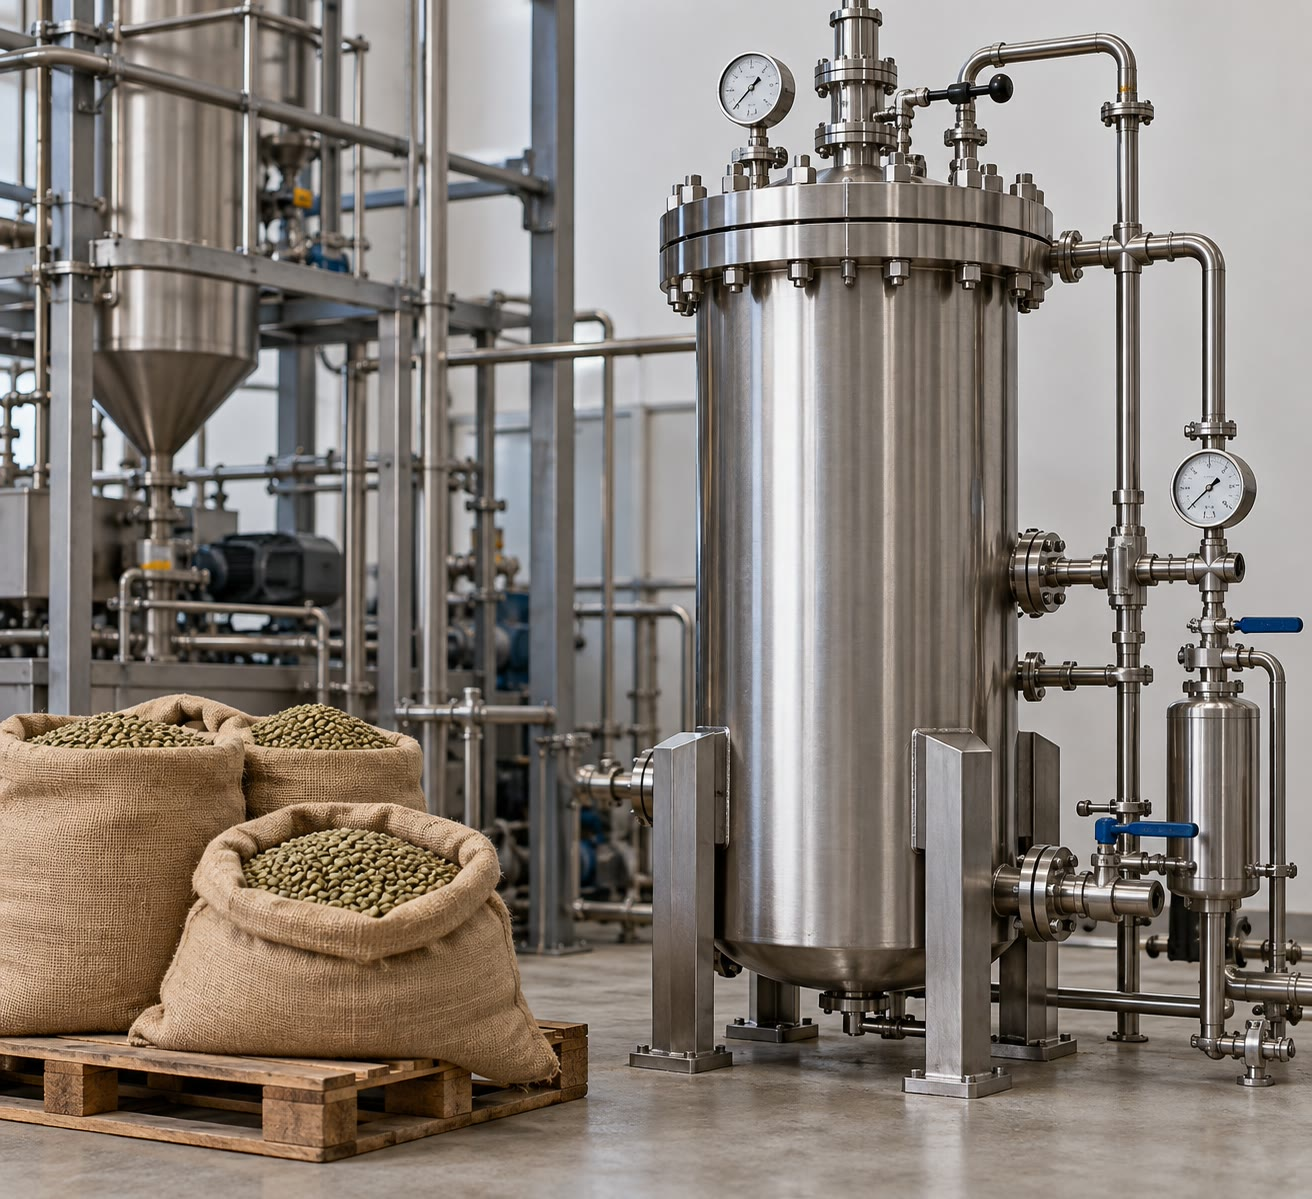
\includegraphics[width=0.45\linewidth,height=6cm,keepaspectratio]{images/book1/ai/g12-scco2-vessel.jpg}

{\small Une cuve d'\omterm{def:g10:chemical-species:extraction}{extraction} sous haute pression, dans laquelle du
dioxyde de carbone supercritique remplace un \omterm{def:g6:solutions-and-solubility:solute}{solvant} organique.}
\end{omfigure}

\section{Exercices}

\begin{exercise}[$\star$]\label{exo:g12:synthesis-strategy:1}
On peut fabriquer l'éthanol par \omterm{def:g11:dissolution:solvation}{hydratation} de l'éthène,
\ce{C2H4 + H2O -> C2H5OH},
ou par fermentation du glucose, \ce{C6H12O6 -> 2C2H5OH + 2CO2}. Calculer
l'\omterm{def:g12:synthesis-strategy:atom-economy}{économie d'atomes} de chacune de ces voies.
\end{exercise}

\begin{exercise}[$\star$]\label{exo:g12:synthesis-strategy:2}
Dans le schéma du dipeptide de ce chapitre, nommer l'étape où chaque
\omterm{def:g12:synthesis-strategy:protecting-group}{groupe protecteur} est mis en place, et l'étape où il est retiré.
\end{exercise}

\begin{exercise}[$\star$]\label{exo:g12:synthesis-strategy:3}
Une usine remplace un \omterm{def:g6:solutions-and-solubility:solute}{solvant} chloré par de l'eau dans l'une de ses
réactions. Quel principe de la \omterm{def:g12:synthesis-strategy:green-chemistry}{chimie verte} applique-t-elle~?
\end{exercise}

\begin{exercise}[$\star$]\label{exo:g12:synthesis-strategy:4}
Pourquoi un excès d'éthanol augmente-t-il le \omterm{def:g10:synthesis-yield:yield}{rendement} d'une
estérification, alors qu'un \omterm{def:g12:catalysis:catalyst}{catalyseur} ne le fait pas~?
\end{exercise}

\begin{exercise}[$\star$]\label{exo:g12:synthesis-strategy:5}
Le borohydrure de sodium réduit les \omterm{def:g11:functional-groups:carbonyl}{aldéhydes} et les \omterm{def:g11:functional-groups:carbonyl}{cétones}, pas les
\omterm{def:g11:functional-groups:carboxylic-acid}{esters}. Sa réaction avec le 4-oxopentanoate de méthyle (une \omterm{def:g11:functional-groups:carbonyl}{cétone} et un
\omterm{def:g11:functional-groups:carboxylic-acid}{ester}) est-elle \omterm{def:g12:synthesis-strategy:chemoselective}{chimiosélective}~? Quel groupe est transformé~?
\end{exercise}

\begin{exercise}[$\star\star$]\label{exo:g12:synthesis-strategy:6}
Une \omterm{def:g10:the-mole:amount}{mole} d'acide éthanoïque et une \omterm{def:g10:the-mole:amount}{mole} d'éthanol donnent
\qty{0.67}{mol} d'\omterm{def:g11:functional-groups:carboxylic-acid}{ester} à l'équilibre. Proposer deux moyens d'augmenter
cette quantité, et un moyen de l'atteindre plus vite.
\end{exercise}

\begin{exercise}[$\star\star$]\label{exo:g12:synthesis-strategy:7}
On traite le 4-oxopentanoate de méthyle, \ce{CH3-CO-CH2-CH2-CO-O-CH3},
une fois par le borohydrure de sodium, une fois par un excès d'hydrure
de lithium et d'aluminium, qui réduit l'\omterm{def:g11:functional-groups:carboxylic-acid}{ester} en deux \omterm{def:g11:functional-groups:alcohol}{alcools}. Écrire
chaque produit.
\end{exercise}

\begin{exercise}[$\star\star$]\label{exo:g12:synthesis-strategy:8}
Sur le diagramme en barres des \omterm{def:g12:synthesis-strategy:atom-economy}{économies d'atomes}, quelles réactions
conservent plus des trois quarts des \omterm{def:g7:atoms-and-molecules:atom}{atomes}~? Par quel facteur la voie
en trois étapes vers l'ibuprofène est-elle meilleure que celle en six
étapes~?
\end{exercise}

\begin{exercise}[$\star\star$]\label{exo:g12:synthesis-strategy:9}
L'aspirine est fabriquée selon \ce{C7H6O3 + C4H6O3 -> C9H8O4 + C2H4O2}.
Calculer son \omterm{def:g12:synthesis-strategy:atom-economy}{économie d'atomes} et la masse de sous-produit par
kilogramme d'aspirine.
\end{exercise}

\begin{exercise}[$\star\star$]\label{exo:g12:synthesis-strategy:10}
Pourquoi chauffe-t-on une \omterm{def:g10:synthesis-yield:synthesis}{synthèse} à reflux plutôt que dans un ballon
ouvert~? Lequel des deux, la vitesse ou le \omterm{def:g10:synthesis-yield:yield}{rendement}, le chauffage
améliore-t-il~?
\end{exercise}

\begin{exercise}[$\star\star$]\label{exo:g12:synthesis-strategy:11}
Sur la figure des deux voies vers l'ibuprofène, compter les étapes et
dire quels principes de la \omterm{def:g12:synthesis-strategy:green-chemistry}{chimie verte} la nouvelle voie applique. En
citer trois.
\end{exercise}

\begin{exercise}[$\star\star\star$]\label{exo:g12:synthesis-strategy:12}
Une \omterm{def:g10:synthesis-yield:synthesis}{synthèse} en trois étapes a des \omterm{def:g10:synthesis-yield:yield}{rendements} de \qty{80}{\percent},
\qty{70}{\percent} et \qty{90}{\percent}. Calculer le \omterm{def:g10:synthesis-yield:yield}{rendement} global.
Quelle quantité de \omterm{def:g7:chemical-reactions:reactant}{réactif} de départ faut-il pour obtenir
\qty{0.10}{mol} de produit final, une \omterm{def:g10:the-mole:amount}{mole} de \omterm{def:g7:chemical-reactions:reactant}{réactif} de départ donnant
au mieux une \omterm{def:g10:the-mole:amount}{mole} de produit~?
\end{exercise}

\begin{exercise}[$\star\star\star$]\label{exo:g12:synthesis-strategy:13}
Planifier la \omterm{def:g10:synthesis-yield:synthesis}{synthèse} du dipeptide Ala--Gly (l'acide de l'alanine lié à
l'\omterm{def:g11:functional-groups:amine}{amine} de la glycine)~: quels groupes faut-il protéger, et combien
d'étapes le plan comporte-t-il~?
\end{exercise}

\begin{exercise}[$\star\star\star$]\label{exo:g12:synthesis-strategy:14}
Une entreprise qualifie son procédé de «~vert~» parce qu'il utilise un
\omterm{def:g12:catalysis:catalyst}{catalyseur}. Le procédé fonctionne à \qty{250}{\celsius} dans le benzène,
un \omterm{def:g6:solutions-and-solubility:solute}{solvant} toxique, et son \omterm{def:g12:synthesis-strategy:atom-economy}{économie d'atomes} est de \qty{35}{\percent}.
Juger cette affirmation, principe par principe.
\end{exercise}

\begin{exercise}[$\star\star\star$]\label{exo:g12:synthesis-strategy:15}
On extrait la caféine des grains de café soit avec le dichlorométhane,
un \omterm{def:g6:solutions-and-solubility:solute}{solvant} chloré volatil, soit avec du dioxyde de carbone supercritique
à environ \qty{40}{\celsius} et \qty{100}{bar}. Expliquer pourquoi le
second est supercritique, pourquoi il exige une cuve résistante, et
donner deux avantages qu'il présente par rapport au premier.
\end{exercise}

\section{Problème~: deux voies vers l'ibuprofène}

\begin{problem}[{Problème du week-end --- quelle masse de déchets la voie
en trois étapes évite-t-elle par tonne d'ibuprofène~?}]
\label{pb:g12:synthesis-strategy:1}
% ledger: ibu:boots-ae, ibu:bhc-ae, ibu:boots-steps, ibu:bhc-steps, aw:C, aw:H, aw:O, aw:N, aw:Cl, aw:Na
L'ancienne voie vers l'ibuprofène \ce{C13H18O2} compte six étapes.
Additionnés, ses \omterm{def:g7:chemical-reactions:reactant}{réactifs} sont \ce{C10H14}, \ce{C4H6O3},
\ce{C4H7ClO2}, \ce{C2H5ONa}, un acide compté comme \ce{H3O},
\ce{NH3O} et deux \ce{H2O}. La nouvelle voie compte trois étapes~:
\[
  \ce{C10H14 + C4H6O3 + H2 + CO -> C13H18O2 + C2H4O2} .
\]

\medskip
\noindent\textbf{Partie I --- Les équations.}
\begin{enumerate}
  \item Vérifier que l'équation de la nouvelle voie est ajustée pour le
        carbone, l'hydrogène et l'oxygène.
  \item Nommer le sous-produit de la nouvelle voie.
  \item Dans l'ancienne voie, quels éléments des \omterm{def:g7:chemical-reactions:reactant}{réactifs} se retrouvent
        entièrement dans les déchets~?
  \item Laquelle des deux voies utilise des \omterm{def:g12:catalysis:catalyst}{catalyseurs}~? Quel principe
        cela applique-t-il~?
\end{enumerate}

\medskip
\noindent\textbf{Partie II --- Les \omterm{def:g12:synthesis-strategy:atom-economy}{économies d'atomes}.}
\begin{enumerate}[resume]
  \item Calculer la \omterm{def:g10:the-mole:molar-mass}{masse molaire} de l'ibuprofène.
  \item Calculer la somme des \omterm{def:g10:the-mole:molar-mass}{masses molaires} des \omterm{def:g7:chemical-reactions:reactant}{réactifs} de l'ancienne
        voie.
  \item En déduire son \omterm{def:g12:synthesis-strategy:atom-economy}{économie d'atomes}.
  \item Calculer la somme des \omterm{def:g10:the-mole:molar-mass}{masses molaires} des \omterm{def:g7:chemical-reactions:reactant}{réactifs} de la
        nouvelle voie.
  \item En déduire son \omterm{def:g12:synthesis-strategy:atom-economy}{économie d'atomes}.
  \item Que devient-elle si l'acide éthanoïque est compté comme
        produit~?
\end{enumerate}

\medskip
\noindent\textbf{Partie III --- Les déchets par tonne.}
\begin{enumerate}[resume]
  \item Pour l'ancienne voie, avec un \omterm{def:g10:synthesis-yield:yield}{rendement} de \qty{100}{\percent},
        quelle masse de \omterm{def:g7:chemical-reactions:reactant}{réactifs} achète-t-on par tonne d'ibuprofène~?
  \item Quelle masse de déchets cela donne-t-il par tonne~?
  \item Même question pour la nouvelle voie~: masse de \omterm{def:g7:chemical-reactions:reactant}{réactifs} par
        tonne.
  \item Masse d'acide éthanoïque par tonne.
  \item Quelle masse de déchets par tonne est évitée si l'acide
        éthanoïque est compté comme déchet~?
\end{enumerate}

\medskip
\noindent\textbf{Partie IV --- Les \omterm{def:g10:synthesis-yield:yield}{rendements} et le monde réel.}
\begin{enumerate}[resume]
  \item On suppose que chaque étape a un \omterm{def:g10:synthesis-yield:yield}{rendement} de
        \qty{90}{\percent}.
        Calculer le \omterm{def:g10:synthesis-yield:yield}{rendement} global de l'ancienne voie.
  \item Même question pour la nouvelle voie.
  \item Donner une raison de plus, en dehors de l'équation, pour laquelle
        moins d'étapes signifie moins de déchets.
  \item En pratique, l'acide éthanoïque est récupéré et utilisé. Quelle
        masse de déchets par tonne la nouvelle voie donne-t-elle alors,
        avec un \omterm{def:g10:synthesis-yield:yield}{rendement} de
        \qty{100}{\percent}~?
  \item Donner la réponse finale~: quelle masse de déchets la voie en
        trois étapes évite-t-elle par tonne d'ibuprofène~?
\end{enumerate}
\end{problem}
